\documentclass[crop,tikz]{standalone}
\usetikzlibrary{positioning,arrows,fit,calc}
\pgfdeclarelayer{bg}
\pgfsetlayers{bg,main}
\tikzset{
	>=stealth'
}
\begin{document}
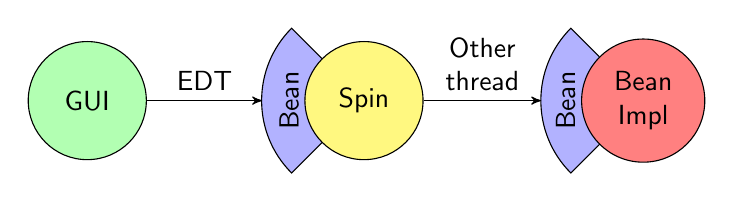
\begin{tikzpicture}[
node distance = 2cm,
every node/.style = {
	font = \sffamily,
	align=center
},
component/.style = {
	circle, 
	draw,
	text width = 1cm,
	minimum width = 1.5cm,
}
]

\node (gui) [component, fill=green!30] {GUI};

\node (spin) [component, fill=yellow!50, right = of gui] {Spin};
\begin{pgfonlayer}{bg}
\filldraw[fill=blue!30] (spin) -- ++(135:13mm) arc[start angle = 135, end angle=225, radius=13mm] -- ++(225:-13mm) -- (spin) -- cycle;
\end{pgfonlayer}
\node [rotate=90, left = -0.5mm of spin, anchor=south] {Bean};


\node (impl) [component, fill=red!50, right = of spin] {Bean Impl};
\begin{pgfonlayer}{bg}
\filldraw[fill=blue!30] (impl) -- ++(135:13mm) arc[start angle = 135, end angle=225, radius=13mm] -- ++(225:-13mm) -- (impl) -- cycle;
\end{pgfonlayer}
\node [rotate=90, left = -0.5mm of impl, anchor=south] {Bean};

\draw[->] (gui) -- node[above] {EDT} ++(2.22cm,0);
\draw[->] (spin) -- node[above, text width=15mm] {Other \\thread} ++(2.25cm,0);

%\filldraw [fill=red] (spin) -- ++(225:9mm)
%	([shift=(135:9mm)]spin) arc (135:225:9mm)
%      (spin) -- ++(135:9mm);
      
%\draw [] ([shift=(135:9mm)]spin) arc (135:225:9mm); 


\end{tikzpicture}

\end{document}